\begin{frame}
  \frametitle{Parallel planes}
\begin{columns}
\column{0.4\textwidth}
\psfrag{cP1}{$\mathcal{P}_1$}
\psfrag{cP2}{$\mathcal{P}_2$}
\psfrag{P1}{$P_1(\textbf{r}_1)$}
\psfrag{P2}{$P_2(\textbf{r}_2)$}
\psfrag{n1}{$\textbf{n}_1$}
\psfrag{n2}{$\textbf{n}_2$}
\psfrag{r12}{$\textbf{r}_2\!-\!\textbf{r}_1$}
\psfrag{proj}{$\textbf{\text{proj}}_{\bm{n}_1} (\textbf{r}_1\!-\!\textbf{r}_0)$}
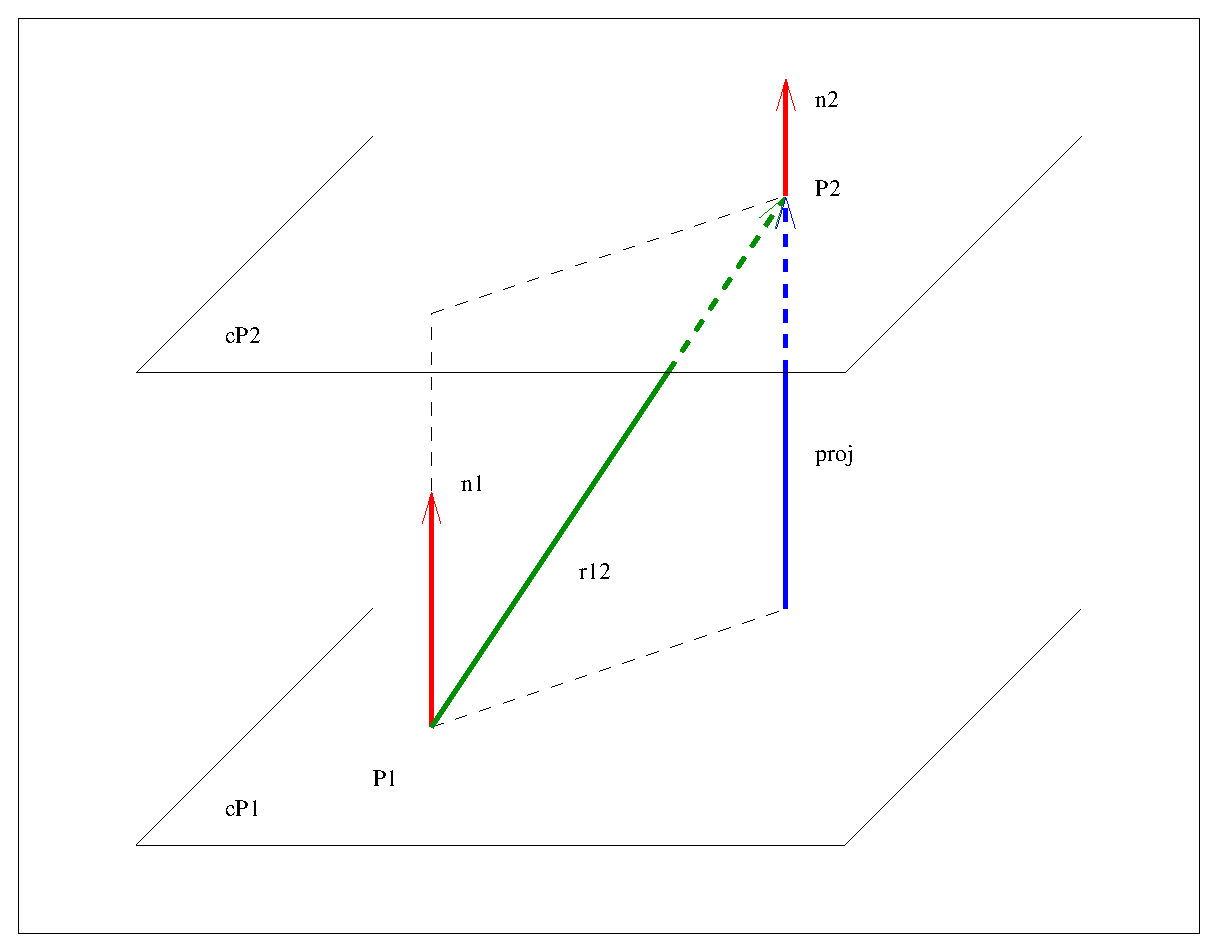
\includegraphics[height=1.4in]{../../modules/vectors/pictures/ok-parallel_plane_plane.eps}
\column{0.6\textwidth}
\begin{itemize}
\item Given: planes $\mathcal{P}_1: \quad (\textbf{r} - \textbf{r}_1) \cdot \textbf{n}_1 = 0$, $\mathcal{P}_2: \quad (\textbf{r} - \textbf{r}_2) \cdot \textbf{n}_2 = 0$
\item Goal: Establish whether planes are parallel, find distance b-n planes.
\end{itemize}
     
\end{columns}
\alert<1->{Parallel} planes: \uncover<2->{$\mathcal{P}_1 || \mathcal{P}_2$ $\Longleftrightarrow$ $\textbf{n}_1$, $\textbf{n}_2$ collinear $\Longleftrightarrow$
$\boxed{\textbf{n}_1 \times \textbf{n}_2 = \textbf{0}}$}
\uncover<3->{
\alert<1->{Distance} between parallel planes: 
$$d(\mathcal{P}_1,\mathcal{P}_2) = |\textbf{\text{proj}}_{\textbf{n}_1} (\textbf{r}_2-\textbf{r}_1)| =\boxed{\frac{|(\textbf{r}_2-\textbf{r}_1)\cdot \textbf{n}_1|}{|\textbf{n}_1|}}$$}
\uncover<4->{
\noindent\alert<1->{Scalar} eq-ns:
$\begin{array}{r@{~}r@{~}c@{~}l} 
\mathcal{P}_1 :& ax+by+cz &=& d_1\\
\mathcal{P}_2 :& ax+by+cz &=& d_2
\end{array}
$ $\boxed{d(\mathcal{P}_1,\mathcal{P}_2) = \frac{|d_2-d_1|}{\sqrt{a^2+b^2+c^2}}}$
}
\end{frame}